\section{ Simulation }

\subsection*{ 1. }

inversion method: calculate cdf by integrating density and invert this cdf.

Calculate the cumulative distribution function F(x) $\rightarrow $ integrate f(x):
\begin{align*}
F\left(x\right)&=\begin{cases}
x^{3}&0\le x\le 1\\
1&x> 1\\
\end{cases}
\end{align*}

inverse function: instead of returning y from x, the inverse function returns x given y: $F^{{-1}}\left(u\right)=\sqrt[3]{u}$ with $u=$ random sample $\in \left[0,1\right]$

\subsection*{ 2. }

\textbf{definitions}

\begin{itemize}
\item  $I_{0}\left(\kappa \right)=$ modified Bessel function of order 0
\item  $\kappa > 0$
\item  density von Mises Distribution: $f\left(x\right)=\frac{e^{{\kappa \cos \left(x\right)}}}{2\pi I_{0}\left(\kappa \right)}$ for $-\pi \le x\le \pi $, density is 0 otherwise
\end{itemize}

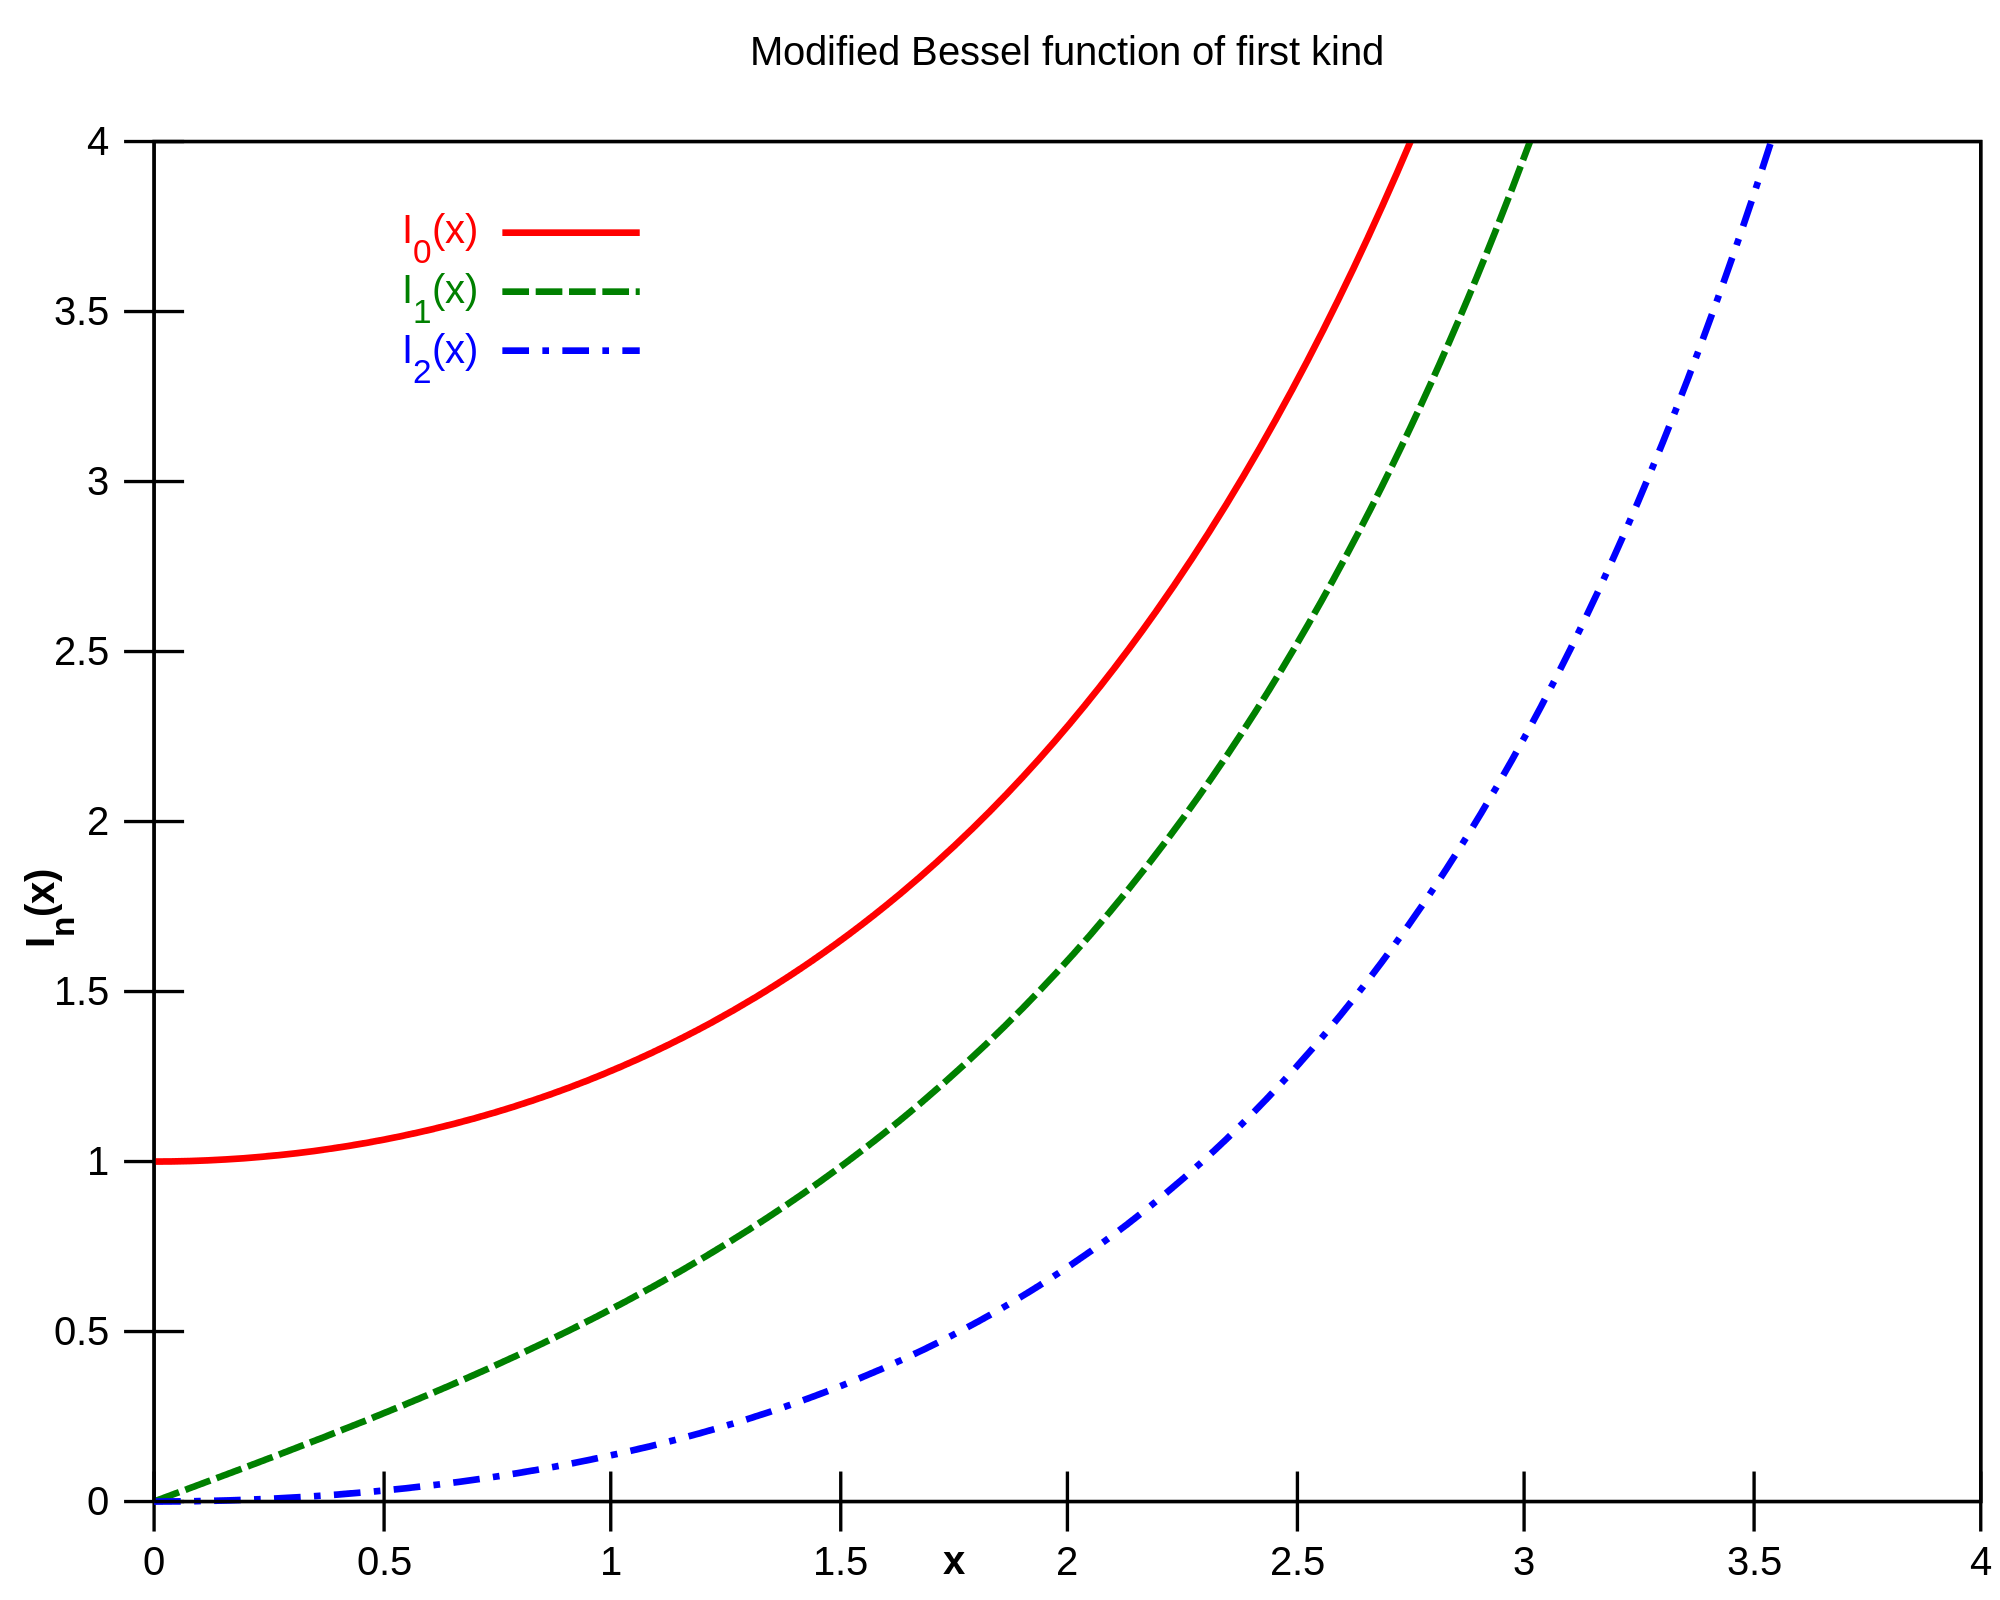
\includegraphics[width=0.65\textwidth]{pics/simulation_2_bessel.png}

\subsubsection*{ (1) }

based on plot: $I_{0}\left(\kappa \right)> 1$
finding extremum $\rightarrow $ derivative:

\begin{align*}
\frac{-K \sin \left(x\right)e^{{\kappa \cos \left(x\right)}}}{2\pi I_{0}\left(\kappa \right)}
\end{align*}
fill in for K=1, since we just want to know the sign: slope is positive for $f'(x)<0$,
0 for $f'(x)=0$ and negative for $f'(x)>0$, hence the maximum is at 0 when $-\pi \le x\le \pi $.

\subsubsection*{ (2) }

\begin{itemize}
\item  find $f_{y}$ such that $f_{y}\sim f_{x}$
\item  find $C\in \mathbb{R}> t$
\item  $C f_{y}\left(x\right)\ge f_{x}\left(x\right), \forall x\in \mathbb{R}$
\item  sample $u$ and $y\rightarrow $ if $u\left(f_{y}\left(y\right)\le f_{x}\left(y\right)\right)$ return y else sample again
\end{itemize}

\begin{align*}
f_{y}\left(y\right)&=\begin{cases}
\frac{\pi }{2}&-\pi < y\le \pi \\
0&otherwise\\
\end{cases}
\end{align*}

\begin{align*}
C = f(0) 2 \pi = \frac{e^{\kappa}}{I_0 (\kappa)}
\end{align*}

\subsection*{ 3 }

\subsubsection*{ (1) }

$F^{-1}(u) = (1-(1-u)^{1/b})^{1/a}$

\subsubsection*{ (2) }

$B\sim Beta\left(|\alpha ,\beta \right)$
\begin{align*}
Pr\left[B^{{\frac{1}{a}}}\le x\right]&=Pr\left[K\le x\right]\\
&=Pr\left[B\le x^{a}\right]\\
&=F_{B}\left(x^{a}\right)\\
&=\int _{0}^{{x^{a}}}f_{B}\left(t\right)dt\\
&=\int _{0}^{x}f_{B}\left(S^{a}\right)as^{{a-1}}ds&& \text{- clean int limits$\rightarrow$  substitute $t$ with $S^{a},a\in \mathbb{N}$ -}\\
&=\int _{0}^{x}\frac{1}{B\left(\alpha ,\beta \right)}\left(1-S^{a}\right)^{{\beta -1}}as^{{\alpha -1}}ds&& \text{-  solve $f_B(S^a)$, $\left(1-S^{a}\right)^{{\beta -1}}as^{{\alpha -1}}\approx f_{K}\left(s\right)$ -}\\
&=Pr\left[K\le x\right]\\
&=F_{k}\left(x\right)
\end{align*}

\subsubsection*{ (3) }

\begin{itemize}
\item  uniform random variable: $u\in \left[0,1\right]$
\item  $x_{K}=\left(1-\left(1-u\right)^{{\frac{1}{b}}}\right)^{{\frac{1}{a}}}$
\item $x_{B}=x^{a}_{K}=\left(1-\left(1-K\right)^{{\frac{1}{b}}}\right) \rightarrow $ given: $\alpha = 1$
\end{itemize}

\subsection*{ 4. }

\begin{align*}
J&=\int _{0}^{1}\int _{0}^{1}e^{\left(x+y\right)^{2}}dydx\\
&=E\left[e\left(x+y\right)^{2}\right]&& \text{-  double integral is like expectation, $x,y\sim $ uniform [0,1] -}\\
&=\int _{0}^{1}\int _{0}^{1}e^{\left(x+y\right)^{2}}f_{x}\left(x\right)f_{y}\left(y\right)dxdy\\
J_{K}&=\frac{1}{K}\sum _{{i=1}}^{K}e^{\left(x_{i}+y_{i}\right)^{2}}
\end{align*}
monte carlo $\rightarrow x_{1},\ldots ,x_{K}y_{1},\ldots ,y_{K}$ generate samples from uniform intervals 
correlation $\left(y_{i,}1-y_{i}\right)< 0$

\begin{align*}
\widehat{J}_{K}&=\frac{1}{K}\sum _{{i=1}}^{K}\frac{1}{2}e^{\left(x_{i}+y_{i}\right)^{2}}+e^{\left(2-x_{i}-y_{i}\right)^{2}}
\end{align*}

negative correlation antithetic $\rightarrow $ see syllabus $\rightarrow $ smaller amount of samples for same conf variables

\subsection*{ 5. }

samples $Z_{1},\ldots ,Z_{K}$

\begin{align*}
\widehat{J}_{K}&=\frac{1}{K}\sum _{i}=1^{K}Z_{i}^{3}e^{{Z_{i}}}&& \text{-  corr(Z, -Z) = E([Z-E(Z)][-Z-E(-Z)]) = -1 -}\\
\widehat{J}_{K}^{a}&=\frac{1}{K}\sum ^{K}\frac{1}{2}\left(Z^{3}_{i}e^{{Z_{i}}}-Z_{i}^{3}e^{{-Z_{i}}}\right)
\end{align*}
monotone, negative correlation $\rightarrow $ lower variance

\subsection*{ 6. }

u is uniformly distributed, $\widetilde{u} = 1-u$ is uniformly distributed. $F_{x}\left(x\right)=1-e^{{-x}}$\\
$x\rightarrow \widetilde{u}=e^{-x}\rightarrow u=1-e^{-x}\rightarrow -\ln \left(1-e^{-x}\right)$\\
$\exp \rightarrow uniform\rightarrow uniform\rightarrow \exp $\\
$corr\left(\widetilde{u},u\right)< 0-\ln \left(\right)\rightarrow corr\left(-\ln \left(\left(\widetilde{u}\right),-\ln \left(u\right)\right)\right)< 0\rightarrow corr\left(x,-\ln \left(1-e^{-x}\right)\right)< 0$

\subsection*{ 7. }

\subsubsection*{ (1) }

\begin{align*}
\prod _{{\{x+y\le t\}}}\left(x+y\right)&=\begin{cases}
1&x+y< t\\
0&x+y> t\\
\end{cases}
\end{align*}
\begin{align*}
Pr\left[x+y\le t\right]&=E\left[\prod _{{\{\}}}\left(x+y\right)\right]
\end{align*}
\begin{align*}
\widehat{J}_{K}&=\frac{1}{K}\sum _{{i=1}}^{K}\prod _{{\{\}}}\left(x_{i}+y_{i}\right)
\end{align*}

\subsubsection*{ (2) }

\textbf{definitions}

\begin{itemize}
\item  $h$ is the indicator function
\item  we leave the {} out the subsript of $\prod _{{\{\}}}$ for clarity
\end{itemize}

\textbf{solution}

\begin{align*}
\widehat{J}_{K}^{{cond}}&=E\left[\prod ^{{\ast }}\left(X+Y\right)\right]\\
&=E\left[E\left[\prod ^{{\ast }}\left(X+Y\right)|X\right]\right]\\
&=E\left[\prod _{{X+Y\le t}}\left(X+Y\right)|X\right]\\
&=E\left[\prod _{{y\le t-x}}\left(Y\right)|X\right]\\
&=G\left(t-x\right)\\
&=Pr\left[y\le t-X|X\right]
\end{align*}
\begin{align*}
J&=E\left[\prod ^{{\ast }}\left(X+Y\right)\right]=E\left[G\left(t-x\right)\right]\\
\widehat{J}_{K}^{{cond}}&=\frac{1}{K}\sum _{{i=1}}^{K}G\left(t-x_{i}\right)&& \text{-  better because only one variable to sample -}
\end{align*}

\subsubsection*{ (3) }

\textbf{definitions}

\begin{itemize}
\item  $u,E\left[h\left(u\right),V,g\left(V\right),E\left(g\left(V\right)\right)\right]$
\end{itemize}

\textbf{solution}

\begin{align*}
E\left[h\left(u\right)\right]&=E\left[h\left(u\right)+\left[g\left(V\right)-E\left(g|V\right)\right]\right]K&& \text{-  $K\in \mathbb{R}$ -}\\
E\left[G\left(t-X\right)\right]&=E\left[G\left(t-X\right)+K\left[X-\mu _{x}\right]\right]&& \text{-  determine K online -}
\end{align*}
\begin{align*}
\widehat{J}_{K}&=\frac{1}{K}\sum _{{i=1}}^{K}\left(G\left(t-x_{t}\right)+K\left(x_{i}-\mu _{x}\right)\right)
\end{align*}

\pagebreak